% ============================================================
%  Sensor Selection Problem for Smart Systems
%  Optimization Techniques -- IIITDM Kancheepuram
%  Authors: Anjaninithin Chalamchala (CS23B1102)
%           P.L.N. Nikhil (CS23B1038)
% ============================================================
\documentclass[12pt,a4paper]{article}

% ---------- Packages ----------
\usepackage[utf8]{inputenc}
\usepackage{amsmath,amssymb,mathrsfs}
\usepackage{graphicx}
\usepackage[top=1in,bottom=1in,left=1in,right=1in]{geometry}
\usepackage[colorlinks=true,linkcolor=blue,citecolor=blue,urlcolor=blue]{hyperref}
\usepackage{booktabs}
\usepackage{caption}
\usepackage{float}
\usepackage{setspace}
\usepackage{array}
\usepackage{multirow}
\usepackage{xcolor}
\usepackage{titlesec}
\usepackage{parskip}

\onehalfspacing

% ---------- Section formatting ----------
\titleformat{\section}{\large\bfseries}{\thesection.}{0.5em}{}
\titleformat{\subsection}{\normalsize\bfseries}{\thesubsection}{0.5em}{}

% ============================================================
\begin{document}

% ============================================================
%  TITLE PAGE
% ============================================================
\begin{titlepage}
  \centering

  \includegraphics[width=0.22\textwidth]{images/iiit_logo.jpg}\\[0.4cm]

  {\large\bfseries Indian Institute of Information Technology,\\
  Design and Manufacturing Kancheepuram}\\[0.15cm]
  {\normalsize Chennai -- 600127, Tamil Nadu, India}\\[0.3cm]

  \noindent\rule{\linewidth}{1.5pt}\\[0.2cm]
  {\normalsize\itshape Department of Computer Science and Engineering\\
  Optimization Techniques (CS3001)}\\[0.2cm]
  \noindent\rule{\linewidth}{0.8pt}\\[0.8cm]

  {\LARGE\bfseries Sensor Selection Problem\\[0.3cm]
  for Smart Systems}\\[1.0cm]

  \noindent\rule{0.6\linewidth}{0.4pt}\\[0.5cm]

  {\normalsize
  \begin{tabular}{ll}
    \textbf{Team Member 1:} & Anjaninithin Chalamchala \\
                            & Roll No.\ CS23B1102 \\[0.4cm]
    \textbf{Team Member 2:} & P.L.N.\ Nikhil \\
                            & Roll No.\ CS23B1038 \\
  \end{tabular}}\\[0.8cm]

  \noindent\rule{0.6\linewidth}{0.4pt}\\[0.5cm]

  {\normalsize Academic Year 2024--25, Even Semester}\\[0.2cm]
  {\normalsize\today}

  \vfill

  {\small\textbf{Repository:}\\[0.15cm]
  \url{https://github.com/Nithinchalamchala/Sensor_Selection_Optimization}}\\[0.4cm]

\end{titlepage}

% ============================================================
%  ABSTRACT
% ============================================================
\begin{abstract}
\noindent
This report presents a comprehensive study of the \emph{Sensor Selection Problem} (SSP) for a smart building environment modelled as a $50 \times 50$ grid.
The objective is to choose an optimal subset from $N = 150$ candidate sensors of three heterogeneous types---motion, thermal, and acoustic---so as to simultaneously maximise weighted coverage of priority zones, minimise deployment cost, and minimise redundant overlap, subject to hard budget, redundancy, and connectivity constraints.

Four metaheuristic algorithms are designed, implemented, and compared: a Genetic Algorithm (GA), Simulated Annealing (SA), Binary Particle Swarm Optimisation (BPSO), and a Hybrid SA-GA (SAGA).
Line-of-sight visibility between sensors and grid cells is computed via the Bresenham rasterisation algorithm, and five rectangular obstacle walls are incorporated into the building model.
Eight zones with distinct priority weights are defined, with six zones classified as critical and requiring redundant sensor coverage.

Experimental results show that all four algorithms achieve feasible solutions with coverage exceeding 97\%.
The GA attains the best combined fitness ($-0.5261$) by deploying only 21 sensors at 12.9\% of total cost, while the BPSO achieves the highest raw coverage (99.08\%) at the expense of higher cost.
Sensitivity analyses over budget levels, objective weights, and candidate pool size confirm the robustness of the formulation and reveal that coverage plateaus beyond a 50\% budget and that the critical jump in coverage occurs between $N = 50$ and $N = 100$ candidate sensors.
\end{abstract}

\tableofcontents
\newpage

% ============================================================
%  SECTION 1 -- CHOSEN PROBLEM AND METHODS
% ============================================================
\section{Chosen Problem and Methods}

\subsection{Problem Context}

The proliferation of Internet-of-Things (IoT) devices in modern buildings has created a pressing need for principled methods to decide \emph{which} sensors to deploy and \emph{where}.
Deploying every available sensor is economically infeasible and operationally wasteful; deploying too few leaves critical areas unmonitored.
The Sensor Selection Problem (SSP) formalises this trade-off as a binary combinatorial optimisation problem: given a set of candidate sensor locations and types, select a subset that maximises coverage quality while respecting budget and reliability constraints.

In this project the environment is a $50 \times 50$ unit smart building floor plan containing eight functionally distinct zones, five rectangular obstacle walls that block line-of-sight, and $N = 150$ pre-placed candidate sensors drawn from three sensor types.
Each sensor type has a characteristic detection radius and unit cost.
The problem is inherently multi-objective---coverage, cost, and overlap are competing criteria---and the feasible region is defined by three hard constraints: a total budget cap, a redundancy requirement for critical zones, and a connectivity requirement ensuring the selected sensors form a single connected communication network.

\subsection{Why Metaheuristics?}

The SSP belongs to the class of NP-hard combinatorial problems.
With $N = 150$ binary decision variables the search space contains $2^{150} \approx 1.4 \times 10^{45}$ candidate solutions, making exhaustive enumeration completely intractable.
Classical branch-and-bound methods scale poorly with problem size, and the non-linear, non-convex nature of the combined fitness function (which includes a line-of-sight computation and a connectivity check) precludes the direct application of gradient-based solvers.
Metaheuristic algorithms---which trade optimality guarantees for practical scalability---are therefore the natural choice.

\subsection{Selected Algorithms}

Four algorithms are implemented and compared in this study.

\textbf{Genetic Algorithm (GA).}
The GA is a population-based evolutionary algorithm that mimics natural selection.
It maintains a population of candidate solutions (chromosomes), applies selection, crossover, and mutation operators to generate offspring, and retains the fittest individuals across generations.
The GA is well-suited to combinatorial problems because it operates directly on binary strings and can exploit building-block structure through crossover.

\textbf{Simulated Annealing (SA).}
SA is a single-solution trajectory method inspired by the annealing process in metallurgy.
Starting from a random feasible solution, it iteratively proposes small perturbations and accepts improvements unconditionally while accepting deteriorations with a probability that decreases as a ``temperature'' parameter is gradually lowered.
This controlled acceptance of worse solutions allows SA to escape local optima.

\textbf{Binary Particle Swarm Optimisation (BPSO).}
PSO is a swarm-intelligence algorithm in which a population of particles moves through the search space guided by their own best-known position and the swarm's global best.
The binary variant uses a sigmoid transfer function to map continuous velocity values to bit-flip probabilities, making it applicable to binary decision variables.

\textbf{Hybrid SAGA.}
The hybrid algorithm combines the global exploration strength of the GA with the local refinement capability of SA.
Phase~1 runs the GA for 150 generations to obtain a high-quality initial solution; Phase~2 applies SA for 30\,000 iterations starting from the GA's best solution, polishing it further.
This two-phase strategy aims to capture the benefits of both paradigms.

% ============================================================
%  SECTION 2 -- MATHEMATICAL FORMULATION
% ============================================================
\section{Mathematical Formulation}

\subsection{Decision Variables}

Let $\mathcal{S} = \{1, 2, \ldots, N\}$ denote the index set of $N = 150$ candidate sensors.
The decision variable for sensor $i$ is:
\begin{equation}
  x_i \in \{0, 1\}, \quad i = 1, \ldots, N,
\end{equation}
where $x_i = 1$ indicates that sensor $i$ is selected for deployment and $x_i = 0$ indicates it is not.
The complete solution is represented as a binary vector $\mathbf{x} = (x_1, x_2, \ldots, x_N)^{\top} \in \{0,1\}^N$.

\subsection{Sensor Model}

Three sensor types are available, each characterised by a detection radius $r_t$ and a unit deployment cost $c_t$:

\begin{table}[H]
  \centering
  \caption{Sensor type parameters.}
  \label{tab:sensor_types}
  \begin{tabular}{lccc}
    \toprule
    \textbf{Type} & \textbf{Symbol} & \textbf{Radius} $r_t$ & \textbf{Cost} $c_t$ \\
    \midrule
    Motion   & M & 6  & 10 \\
    Thermal  & T & 8  & 18 \\
    Acoustic & A & 10 & 25 \\
    \bottomrule
  \end{tabular}
\end{table}

A grid cell $p$ is said to be \emph{covered} by sensor $i$ of type $t$ if and only if two conditions hold simultaneously:
\begin{enumerate}
  \item The Euclidean distance satisfies $\|p - s_i\|_2 \leq r_t$, where $s_i$ is the grid position of sensor $i$.
  \item There exists an unobstructed line-of-sight path from $s_i$ to $p$, verified using the Bresenham line-drawing algorithm: the path is blocked if any intermediate grid cell lies inside one of the five rectangular obstacle walls.
\end{enumerate}

The building contains five rectangular obstacle walls whose positions are fixed.
These walls create shadow regions that no sensor can cover from the opposite side, adding a non-trivial geometric structure to the coverage computation.

\subsection{Objective Functions}

Three objectives are defined.

\textbf{Objective 1 -- Weighted Coverage (maximise).}
Let $\mathcal{G}$ denote the set of all grid cells and $w(p)$ the priority weight of the zone containing cell $p$.
The weighted coverage fraction is:
\begin{equation}
  f_1(\mathbf{x}) = \frac{\displaystyle\sum_{p \in \mathcal{G}} w(p) \cdot \mathbf{1}\!\left[\exists\, i : x_i = 1 \wedge p \in \text{cov}(i)\right]}
                        {\displaystyle\sum_{p \in \mathcal{G}} w(p)},
  \label{eq:f1}
\end{equation}
where $\text{cov}(i)$ is the set of cells visible from sensor $i$ within its detection radius, and $\mathbf{1}[\cdot]$ is the indicator function.
Higher-priority zones contribute more to the numerator, so the objective rewards covering critical areas.

\textbf{Objective 2 -- Normalised Cost (minimise).}
The normalised deployment cost is:
\begin{equation}
  f_2(\mathbf{x}) = \frac{\displaystyle\sum_{i=1}^{N} c_i\, x_i}{\displaystyle\sum_{i=1}^{N} c_i},
  \label{eq:f2}
\end{equation}
where $c_i$ is the cost of sensor $i$ (determined by its type).
Normalisation by the total possible cost places $f_2$ in $[0, 1]$.

\textbf{Objective 3 -- Coverage Overlap (minimise).}
Redundant coverage wastes sensor capacity.
Let $v(p, \mathbf{x})$ denote the number of selected sensors that cover cell $p$.
The overlap fraction is:
\begin{equation}
  f_3(\mathbf{x}) = \frac{\displaystyle\sum_{p \in \mathcal{G}} \max\!\bigl(v(p,\mathbf{x}) - 1,\; 0\bigr)}
                        {\displaystyle\sum_{p \in \mathcal{G}} v(p,\mathbf{x})},
  \label{eq:f3}
\end{equation}
which equals the fraction of total sensor visits that are redundant (i.e., the cell was already covered by at least one other sensor).

\subsection{Combined Fitness Function}

The three objectives are scalarised into a single minimisation fitness:
\begin{equation}
  F(\mathbf{x}) = -\alpha\, f_1(\mathbf{x}) + \beta\, f_2(\mathbf{x}) + \gamma\, f_3(\mathbf{x}) + \lambda\, P(\mathbf{x}),
  \label{eq:fitness}
\end{equation}
where $\alpha, \beta, \gamma > 0$ are user-specified weights and $P(\mathbf{x}) \geq 0$ is a penalty term for constraint violations (defined in Section~\ref{sec:penalty}).
The negative sign on $f_1$ converts the maximisation of coverage into a minimisation problem consistent with the other two terms.
Default weight values are $\alpha = 0.60$, $\beta = 0.25$, $\gamma = 0.15$, reflecting the primary importance of coverage.

\subsection{Constraints}
\label{sec:constraints}

Three hard constraints are imposed.

\textbf{Constraint C1 -- Budget.}
The total deployment cost must not exceed a budget $B$:
\begin{equation}
  \sum_{i=1}^{N} c_i\, x_i \leq B.
  \label{eq:c1}
\end{equation}
In the default experimental setting $B$ is set to 50\% of the total cost of all candidate sensors.

\textbf{Constraint C2 -- Redundancy for Critical Zones.}
Each critical zone $z \in \mathcal{Z}_{\text{crit}}$ must be covered by at least two distinct selected sensors:
\begin{equation}
  \sum_{i=1}^{N} x_i \cdot \mathbf{1}\!\left[\text{cov}(i) \cap z \neq \emptyset\right] \geq 2, \quad \forall\, z \in \mathcal{Z}_{\text{crit}}.
  \label{eq:c2}
\end{equation}
The six critical zones are: Office~A, Office~B, Lab, Server Room, and Meeting Room (see Table~\ref{tab:zones}).

\textbf{Constraint C3 -- Sensor Connectivity.}
The selected sensors must form a connected communication graph $G(\mathbf{x})$.
An edge exists between sensors $i$ and $j$ if their Euclidean distance satisfies $\|s_i - s_j\|_2 \leq d_{\max}$, with $d_{\max} = 15$ units.
Connectivity is verified by a breadth-first search on $G(\mathbf{x})$:
\begin{equation}
  G(\mathbf{x}) \text{ is connected}, \quad \text{where } G(\mathbf{x}) = \bigl(\{i : x_i = 1\},\; \{(i,j) : \|s_i - s_j\|_2 \leq 15\}\bigr).
  \label{eq:c3}
\end{equation}

\subsection{Penalty Function}
\label{sec:penalty}

Constraint violations are handled via an additive penalty term $P(\mathbf{x})$ in the fitness function.
Let:
\begin{align}
  \delta_B(\mathbf{x})   &= \max\!\left(0,\; \sum_{i} c_i x_i - B\right) / B, \label{eq:pen_budget}\\
  \delta_R(\mathbf{x})   &= \frac{1}{|\mathcal{Z}_{\text{crit}}|}\sum_{z \in \mathcal{Z}_{\text{crit}}} \max\!\left(0,\; 2 - \sum_i x_i \cdot \mathbf{1}[\text{cov}(i)\cap z \neq \emptyset]\right), \label{eq:pen_red}\\
  \delta_C(\mathbf{x})   &= \mathbf{1}\!\left[G(\mathbf{x}) \text{ is disconnected}\right]. \label{eq:pen_conn}
\end{align}
The combined penalty is:
\begin{equation}
  P(\mathbf{x}) = \delta_B(\mathbf{x}) + 0.1\,\delta_R(\mathbf{x}) + 0.05\,\delta_C(\mathbf{x}).
  \label{eq:penalty}
\end{equation}
The budget violation is penalised most heavily because it is a continuous quantity; redundancy and connectivity violations receive smaller coefficients because they are discrete and easier to satisfy once the budget is met.

\begin{table}[H]
  \centering
  \caption{Zone definitions, priority weights, and criticality classification.}
  \label{tab:zones}
  \begin{tabular}{llcc}
    \toprule
    \textbf{Zone} & \textbf{Approximate Location} & \textbf{Weight} $w$ & \textbf{Critical?} \\
    \midrule
    Lobby         & Lower-left entrance area  & 1.0 & No  \\
    Corridor 1    & Horizontal passage        & 1.5 & No  \\
    Office A      & Upper-left office block   & 2.0 & Yes \\
    Office B      & Upper-right office block  & 2.0 & Yes \\
    Lab           & Central laboratory        & 3.0 & Yes \\
    Server Room   & Right-side server area    & 3.5 & Yes \\
    Corridor 2    & Vertical passage          & 1.0 & No  \\
    Meeting Room  & Lower-right meeting area  & 2.5 & Yes \\
    \bottomrule
  \end{tabular}

\end{table}

% ============================================================
%  SECTION 3 -- ALGORITHM IMPLEMENTATION
% ============================================================
\section{Algorithm Implementation}

\subsection{Genetic Algorithm}

The Genetic Algorithm (GA) is a population-based evolutionary search method that operates on a population of binary chromosomes, each representing a candidate sensor selection.
The implementation follows a generational model with elitism, adaptive mutation, and a repair operator to handle constraint violations.

\subsubsection*{Initialisation}

The initial population of 100 chromosomes is generated by randomly setting each bit to 1 with probability $p_{\text{init}} = 0.3$, producing sparse solutions that are unlikely to violate the budget constraint.
Each chromosome is immediately evaluated and repaired if necessary.

\subsubsection*{Selection}

Tournament selection with tournament size $k = 5$ is used.
Five individuals are drawn at random from the population, and the one with the lowest fitness value (best solution) is selected as a parent.
This process is repeated to fill the mating pool.
Tournament selection provides a controllable selection pressure and is robust to fitness scaling issues.

\subsubsection*{Crossover}

Two crossover operators are applied with equal probability:
\begin{itemize}
  \item \textbf{Uniform crossover}: each bit is independently inherited from either parent with probability 0.5.
  \item \textbf{Two-point crossover}: two cut points are chosen uniformly at random, and the segment between them is swapped between the two parents.
\end{itemize}
The overall crossover rate is $p_c = 0.85$; with probability $1 - p_c$ the offspring is a copy of the selected parent.

\subsubsection*{Mutation}

Adaptive bit-flip mutation is applied: each bit is flipped independently with probability $p_m$, which decreases linearly from 0.05 in generation 1 to 0.01 in the final generation.
This schedule provides broad exploration early in the search and fine-grained exploitation later.

\subsubsection*{Repair Operator}

After crossover and mutation, a repair operator enforces feasibility.
If the budget constraint is violated, sensors are removed in ascending order of their cost-to-coverage ratio until the budget is satisfied.
This greedy repair preserves as much coverage as possible while restoring feasibility.

\subsubsection*{Elitism}

The top 5\% of the current population (by fitness) are copied unchanged into the next generation, ensuring that the best solutions found so far are never lost.

\begin{table}[H]
  \centering
  \caption{Genetic Algorithm hyperparameters.}
  \label{tab:ga_params}
  \begin{tabular}{lll}
    \toprule
    \textbf{Parameter} & \textbf{Value} & \textbf{Description} \\
    \midrule
    Population size       & 100          & Number of chromosomes \\
    Generations           & 300          & Maximum iterations \\
    Crossover rate        & 0.85         & Probability of crossover \\
    Mutation rate (start) & 0.05         & Initial bit-flip probability \\
    Mutation rate (end)   & 0.01         & Final bit-flip probability \\
    Tournament size       & 5            & Competitors per selection event \\
    Elitism fraction      & 5\%          & Elite individuals preserved \\
    Crossover operators   & Uniform + Two-point & Applied with equal probability \\
    \bottomrule
  \end{tabular}
\end{table}

\subsection{Simulated Annealing}

Simulated Annealing (SA) is a single-solution stochastic local search algorithm.
Starting from a randomly generated feasible solution, it iteratively proposes a neighbouring solution and accepts or rejects it according to the Metropolis criterion.

\subsubsection*{Neighbourhood Operators}

Two move operators are used in a probabilistic mixture:
\begin{itemize}
  \item \textbf{Bit-flip} (probability 0.70): a single randomly chosen bit is flipped.
    This is a small, local perturbation that allows fine-grained exploration.
  \item \textbf{Block-swap} (probability 0.30): a contiguous block of $k$ bits (with $k$ drawn uniformly from $\{2, 3, 4, 5\}$) is selected at a random position, and each bit in the block is independently flipped with probability 0.5.
    This larger move helps escape deeper local optima.
\end{itemize}

\subsubsection*{Acceptance Criterion}

Let $\Delta F = F(\mathbf{x}') - F(\mathbf{x})$ be the change in fitness when moving from the current solution $\mathbf{x}$ to the proposed solution $\mathbf{x}'$.
The proposed solution is accepted with probability:
\begin{equation}
  P_{\text{accept}} = \begin{cases} 1 & \text{if } \Delta F \leq 0, \\ \exp(-\Delta F / T) & \text{if } \Delta F > 0, \end{cases}
  \label{eq:metropolis}
\end{equation}
where $T$ is the current temperature.

\subsubsection*{Cooling Schedule}

Geometric cooling is used: after each iteration the temperature is updated as $T \leftarrow \alpha_{\text{cool}} \cdot T$ with $\alpha_{\text{cool}} = 0.995$.
Starting from $T_{\text{init}} = 5.0$, the temperature reaches $T_{\min} = 10^{-4}$ after approximately 18\,400 iterations.
The algorithm runs for a maximum of 50\,000 iterations.

\subsubsection*{Reheating}

To avoid premature convergence, a reheating mechanism is incorporated.
If the best fitness has not improved for 500 consecutive iterations (the \emph{patience} threshold), the temperature is multiplied by a reheat factor of 2.
This allows the algorithm to escape stagnation by temporarily increasing the acceptance probability for worse solutions.

\begin{table}[H]
  \centering
  \caption{Simulated Annealing hyperparameters.}
  \label{tab:sa_params}
  \begin{tabular}{lll}
    \toprule
    \textbf{Parameter} & \textbf{Value} & \textbf{Description} \\
    \midrule
    Initial temperature   & 5.0          & Starting $T$ value \\
    Minimum temperature   & $10^{-4}$    & Termination threshold \\
    Cooling rate          & 0.995        & Geometric decay factor $\alpha_{\text{cool}}$ \\
    Maximum iterations    & 50\,000      & Hard iteration limit \\
    Reheat factor         & 2.0          & Temperature multiplier on stagnation \\
    Reheat patience       & 500          & Iterations without improvement before reheat \\
    Bit-flip probability  & 0.70         & Fraction of moves using bit-flip \\
    Block-swap probability& 0.30         & Fraction of moves using block-swap \\
    \bottomrule
  \end{tabular}
\end{table}

\subsection{Binary Particle Swarm Optimisation}

Binary PSO (BPSO) adapts the continuous PSO framework to binary search spaces by using a sigmoid transfer function to convert real-valued velocities into bit-flip probabilities.

\subsubsection*{Velocity and Position Update}

Each particle $k$ maintains a position $\mathbf{x}^{(k)} \in \{0,1\}^N$ and a real-valued velocity $\mathbf{v}^{(k)} \in \mathbb{R}^N$.
At each iteration the velocity is updated as:
\begin{equation}
  v_i^{(k)} \leftarrow \omega\, v_i^{(k)} + c_1 r_1 \bigl(p_i^{(k)} - x_i^{(k)}\bigr) + c_2 r_2 \bigl(g_i - x_i^{(k)}\bigr),
  \label{eq:pso_vel}
\end{equation}
where $\omega$ is the inertia weight, $c_1$ and $c_2$ are cognitive and social acceleration coefficients, $r_1, r_2 \sim \mathcal{U}(0,1)$ are random scalars, $\mathbf{p}^{(k)}$ is the personal best position of particle $k$, and $\mathbf{g}$ is the global best position.
The inertia weight decreases linearly from $\omega_{\max} = 0.9$ to $\omega_{\min} = 0.4$ over the course of the run, balancing exploration and exploitation.

The position is then updated stochastically:
\begin{equation}
  x_i^{(k)} \leftarrow \begin{cases} 1 & \text{with probability } \sigma(v_i^{(k)}), \\ 0 & \text{otherwise,} \end{cases}
  \quad \text{where } \sigma(v) = \frac{1}{1 + e^{-v}}.
  \label{eq:pso_pos}
\end{equation}

\subsubsection*{Levy-Flight Perturbation}

To prevent premature convergence, a Levy-flight perturbation is applied to each particle with probability $p_{\text{levy}} = 0.15$ per iteration.
The perturbation draws a step size from a Levy distribution and flips a corresponding number of bits at random positions.
This introduces occasional large jumps in the search space, helping particles escape local optima.

\subsubsection*{Stagnation Detection}

If the global best fitness has not improved for 30 consecutive iterations, the worst 20\% of particles are re-initialised randomly.
This diversity injection mechanism prevents the swarm from collapsing to a single point.

\begin{table}[H]
  \centering
  \caption{Binary PSO hyperparameters.}
  \label{tab:pso_params}
  \begin{tabular}{lll}
    \toprule
    \textbf{Parameter} & \textbf{Value} & \textbf{Description} \\
    \midrule
    Swarm size            & 80           & Number of particles \\
    Iterations            & 300          & Maximum iterations \\
    Inertia $\omega$ (start) & 0.9       & Initial inertia weight \\
    Inertia $\omega$ (end)   & 0.4       & Final inertia weight \\
    Cognitive coeff.\ $c_1$ & 2.0        & Personal best attraction \\
    Social coeff.\ $c_2$    & 2.0        & Global best attraction \\
    Levy-flight probability & 0.15       & Per-particle perturbation rate \\
    Stagnation limit      & 30           & Iterations before diversity injection \\
    \bottomrule
  \end{tabular}
\end{table}

\subsection{Hybrid SAGA}

The Hybrid SAGA algorithm is a two-phase sequential combination of the GA and SA.
The motivation is that the GA is effective at global exploration and quickly finds a good region of the search space, while SA excels at local refinement within a promising neighbourhood.
By chaining them, the hybrid aims to achieve better final solutions than either algorithm alone.

\subsubsection*{Phase 1: Genetic Algorithm}

The GA is run for 150 generations (half the standalone budget) using the same parameters described in Section~3.1.
At the end of Phase~1, the best chromosome found is extracted as the starting point for Phase~2.

\subsubsection*{Phase 2: Simulated Annealing}

SA is initialised with the GA's best solution and run for 30\,000 iterations.
The temperature schedule is identical to the standalone SA (initial temperature 5.0, cooling rate 0.995), but the starting solution is already of high quality, so the SA spends most of its budget on fine-grained local search rather than broad exploration.

\subsubsection*{Rationale}

The hybrid design addresses a known weakness of each component: the GA can stagnate in a local optimum once the population converges, and SA is sensitive to the quality of its starting point.
By providing SA with a strong initial solution from the GA, the hybrid avoids the slow initial phase that SA would otherwise require when starting from a random solution.

\begin{table}[H]
  \centering
  \caption{Hybrid SAGA hyperparameters.}
  \label{tab:saga_params}
  \begin{tabular}{lll}
    \toprule
    \textbf{Parameter} & \textbf{Value} & \textbf{Description} \\
    \midrule
    GA generations (Phase 1) & 150       & GA budget \\
    SA iterations (Phase 2)  & 30\,000   & SA budget \\
    GA population size       & 100       & Inherited from standalone GA \\
    SA initial temperature   & 5.0       & Inherited from standalone SA \\
    SA cooling rate          & 0.995     & Inherited from standalone SA \\
    Handoff                  & GA best   & SA starts from GA's best solution \\
    \bottomrule
  \end{tabular}
\end{table}

% ============================================================
%  SECTION 4 -- RESULTS AND CONVERGENCE
% ============================================================
\section{Results and Convergence}

\subsection{Quantitative Summary}

Table~\ref{tab:results} summarises the final performance of all four algorithms on the default problem instance ($N = 150$, budget $= 50\%$ of total cost).
All algorithms produce feasible solutions satisfying all three hard constraints.

\begin{table}[H]
  \centering
  \caption{Algorithm performance comparison ($N=150$, budget $= 50\%$).}
  \label{tab:results}
  \begin{tabular}{lrrrrrl}
    \toprule
    \textbf{Algorithm} & \textbf{Fitness} & \textbf{Coverage} & \textbf{Cost} & \textbf{Sensors} & \textbf{Time (s)} & \textbf{Feasible} \\
    \midrule
    GA   & $-0.5261$ & 97.84\% & 12.90\% & 21 & 43.8  & Yes \\
    SA   & $-0.5183$ & 98.05\% & 13.98\% & 24 & 58.4  & Yes \\
    PSO  & $-0.4393$ & 99.08\% & 27.19\% & 44 & 69.5  & Yes \\
    SAGA & $-0.5169$ & 98.45\% & 15.11\% & 23 & 59.9  & Yes \\
    \bottomrule
  \end{tabular}
\end{table}

The GA achieves the best combined fitness of $-0.5261$, deploying only 21 sensors at 12.9\% of the total possible cost.
This reflects the GA's ability to find compact, high-coverage solutions through its crossover and repair operators.
The SA solution is slightly less fit ($-0.5183$) but achieves marginally higher raw coverage (98.05\%) with 24 sensors.
The BPSO solution has the highest raw coverage (99.08\%) but deploys 44 sensors at 27.19\% cost, resulting in the worst combined fitness ($-0.4393$) because the cost and overlap penalties outweigh the coverage gain.
The SAGA hybrid achieves a fitness of $-0.5169$, slightly below the standalone SA, suggesting that the 150-generation GA warm-start does not provide a decisive advantage over SA's own exploration in this instance.

\subsection{Building Map and Sensor Placement}

Figure~\ref{fig:building_map} shows the building floor plan with all eight zones, five obstacle walls, and the candidate sensor positions colour-coded by type.
The zones are rendered with their priority weights, and the obstacles are shown as solid grey rectangles.

\begin{figure}[H]
  \centering
  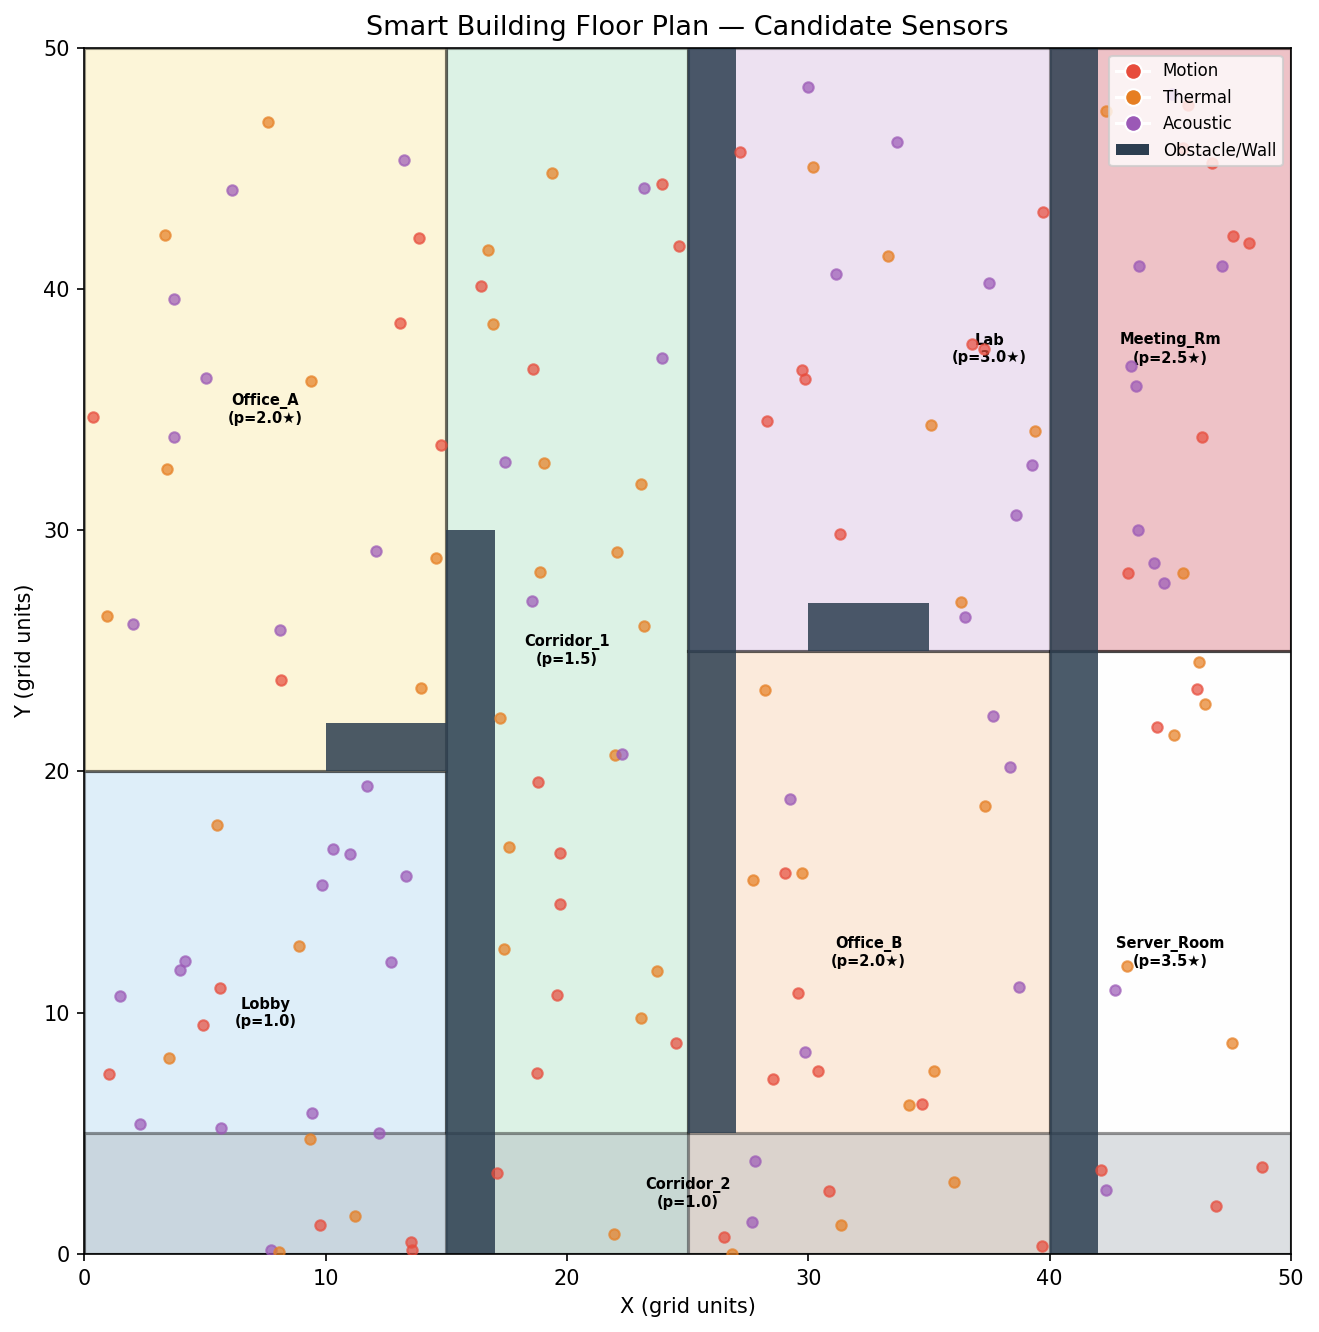
\includegraphics[width=0.85\textwidth]{images/building_map.png}
  \caption{Building floor plan showing zones (colour-coded by priority weight), obstacle walls (grey), and candidate sensor positions (colour-coded by type: motion = blue, thermal = orange, acoustic = green).}
  \label{fig:building_map}
\end{figure}

\subsection{Coverage Heatmaps}

Figures~\ref{fig:cov_ga}--\ref{fig:cov_saga} show the weighted coverage heatmaps produced by each algorithm.
Brighter cells indicate higher coverage weight; dark cells are uncovered.
All four algorithms achieve near-complete coverage of the high-priority zones (Lab, Server Room, Meeting Room), with only marginal differences in the low-priority corridor regions.

\begin{figure}[H]
  \centering
  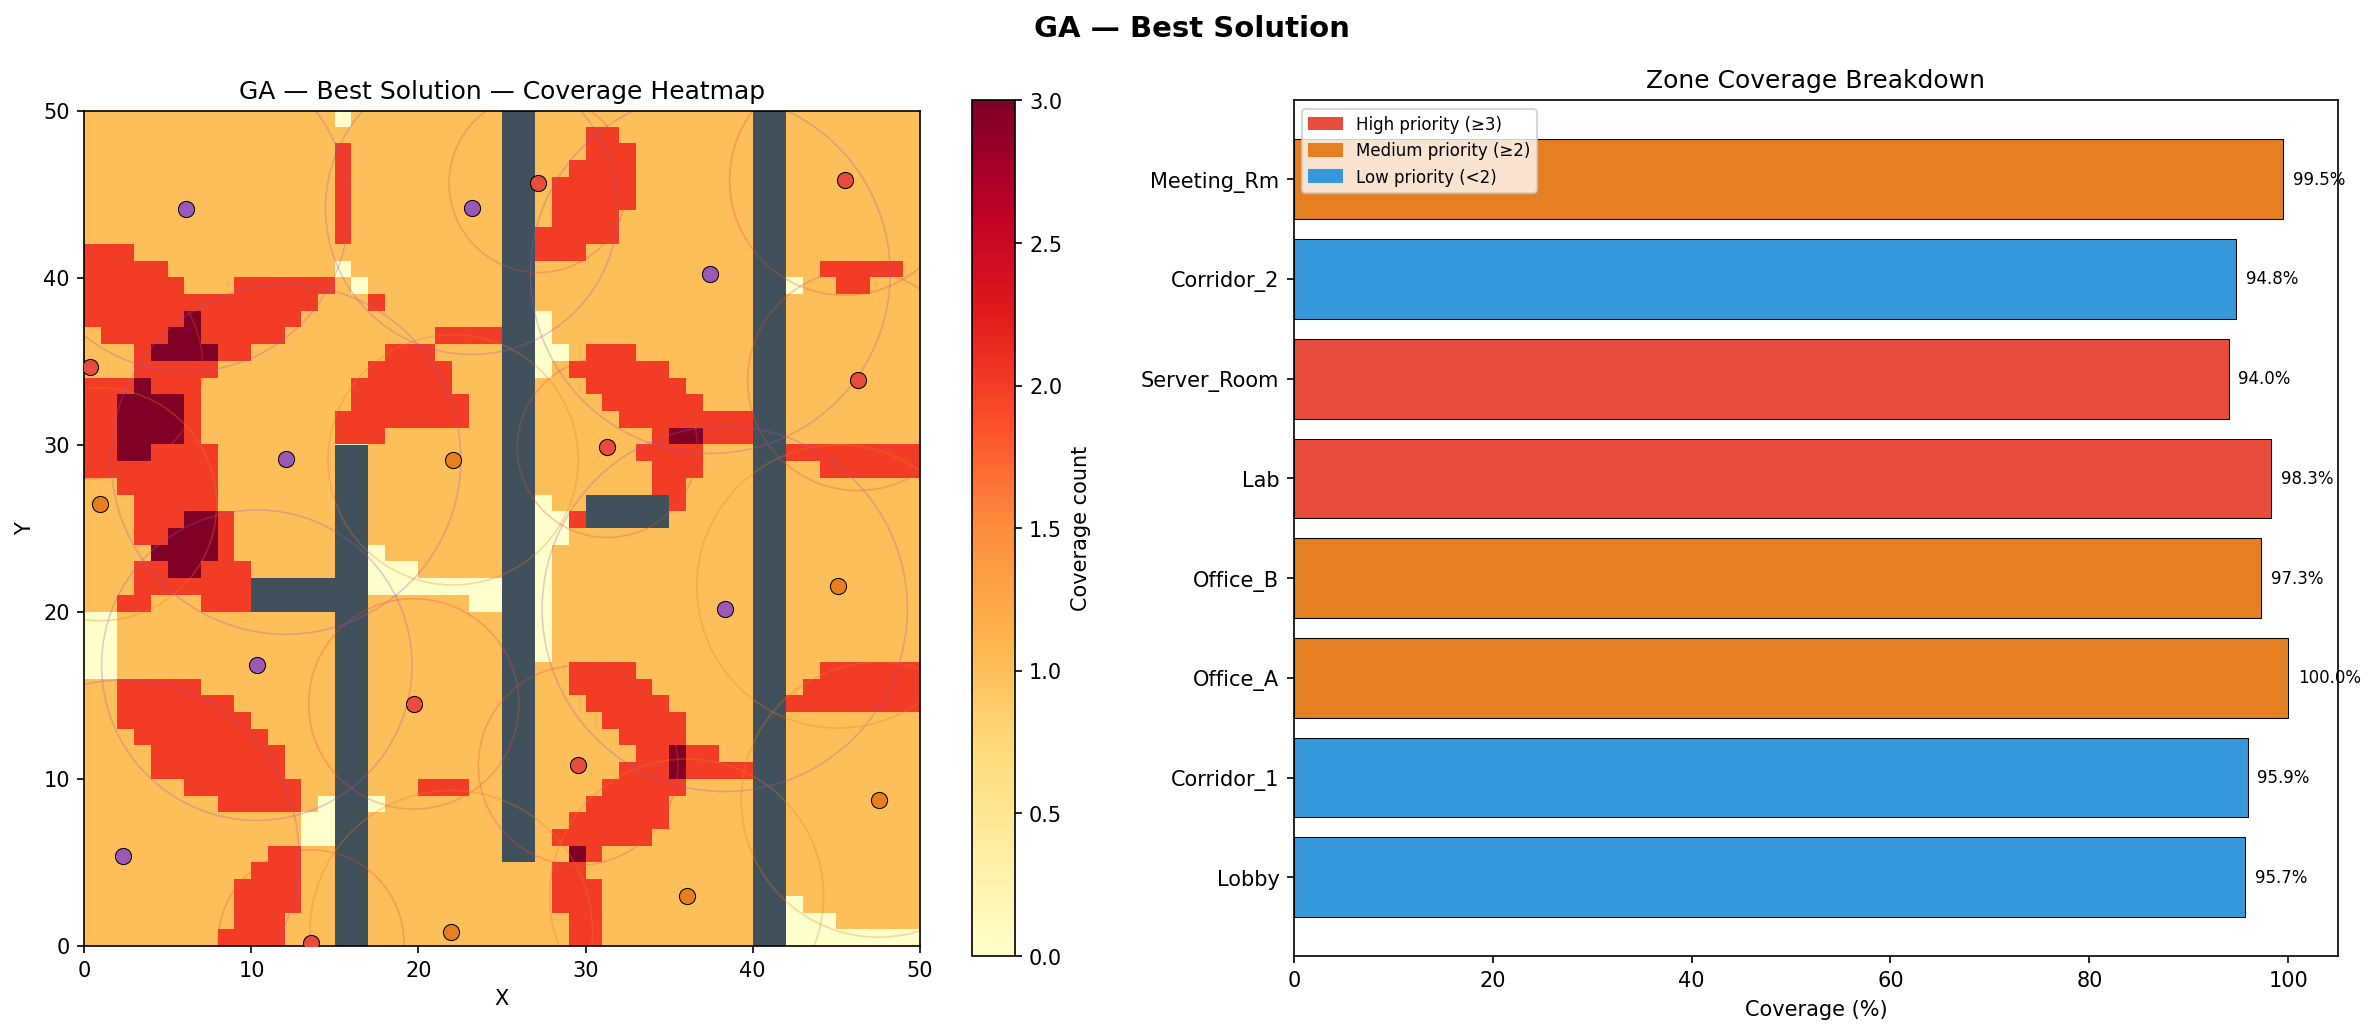
\includegraphics[width=0.80\textwidth]{images/coverage_ga.png}
  \caption{GA coverage heatmap. Selected sensors (21) are marked with crosses. Coverage = 97.84\%.}
  \label{fig:cov_ga}
\end{figure}

\begin{figure}[H]
  \centering
  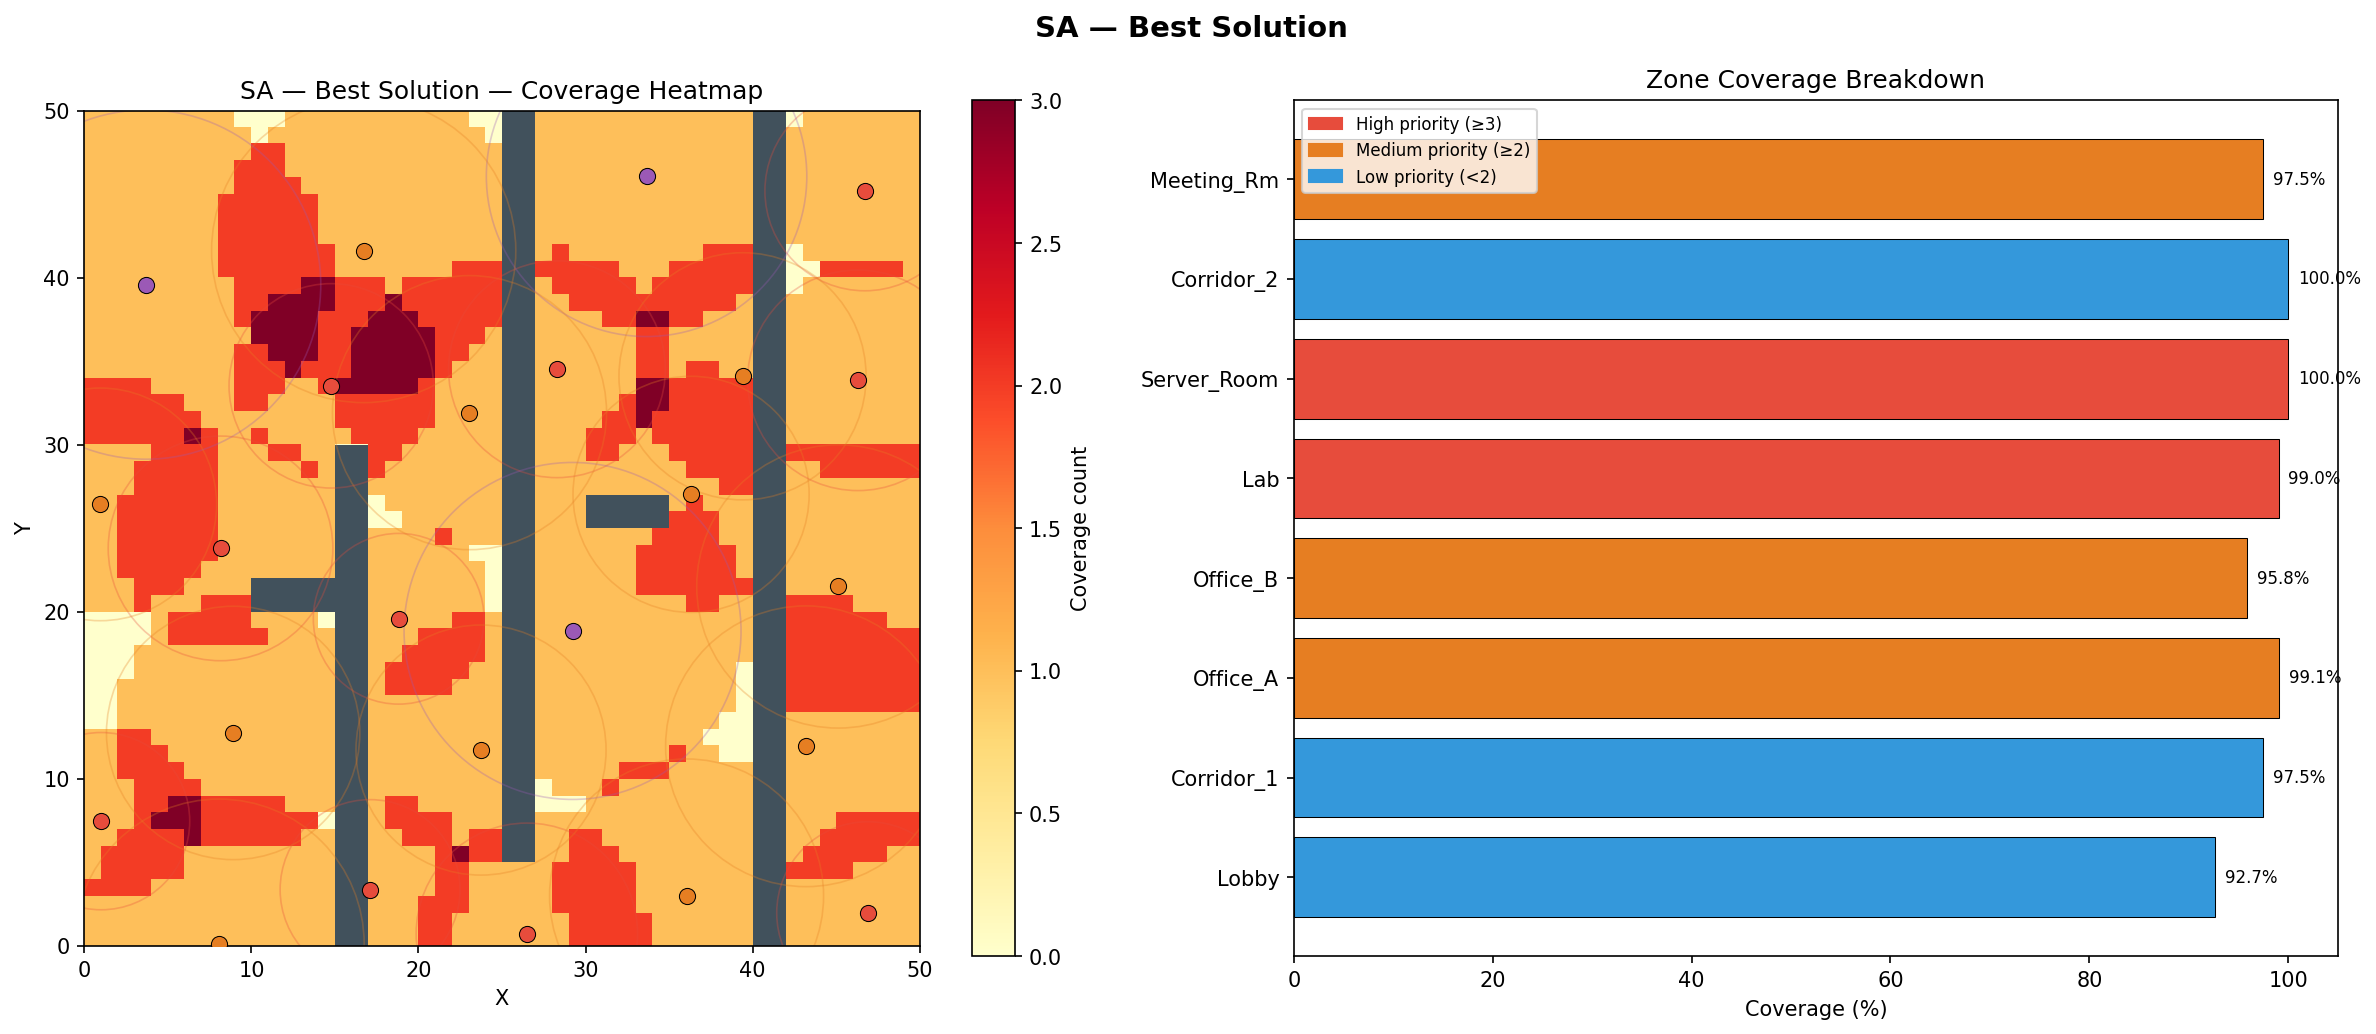
\includegraphics[width=0.80\textwidth]{images/coverage_sa.png}
  \caption{SA coverage heatmap. Selected sensors (24) are marked with crosses. Coverage = 98.05\%.}
  \label{fig:cov_sa}
\end{figure}

\begin{figure}[H]
  \centering
  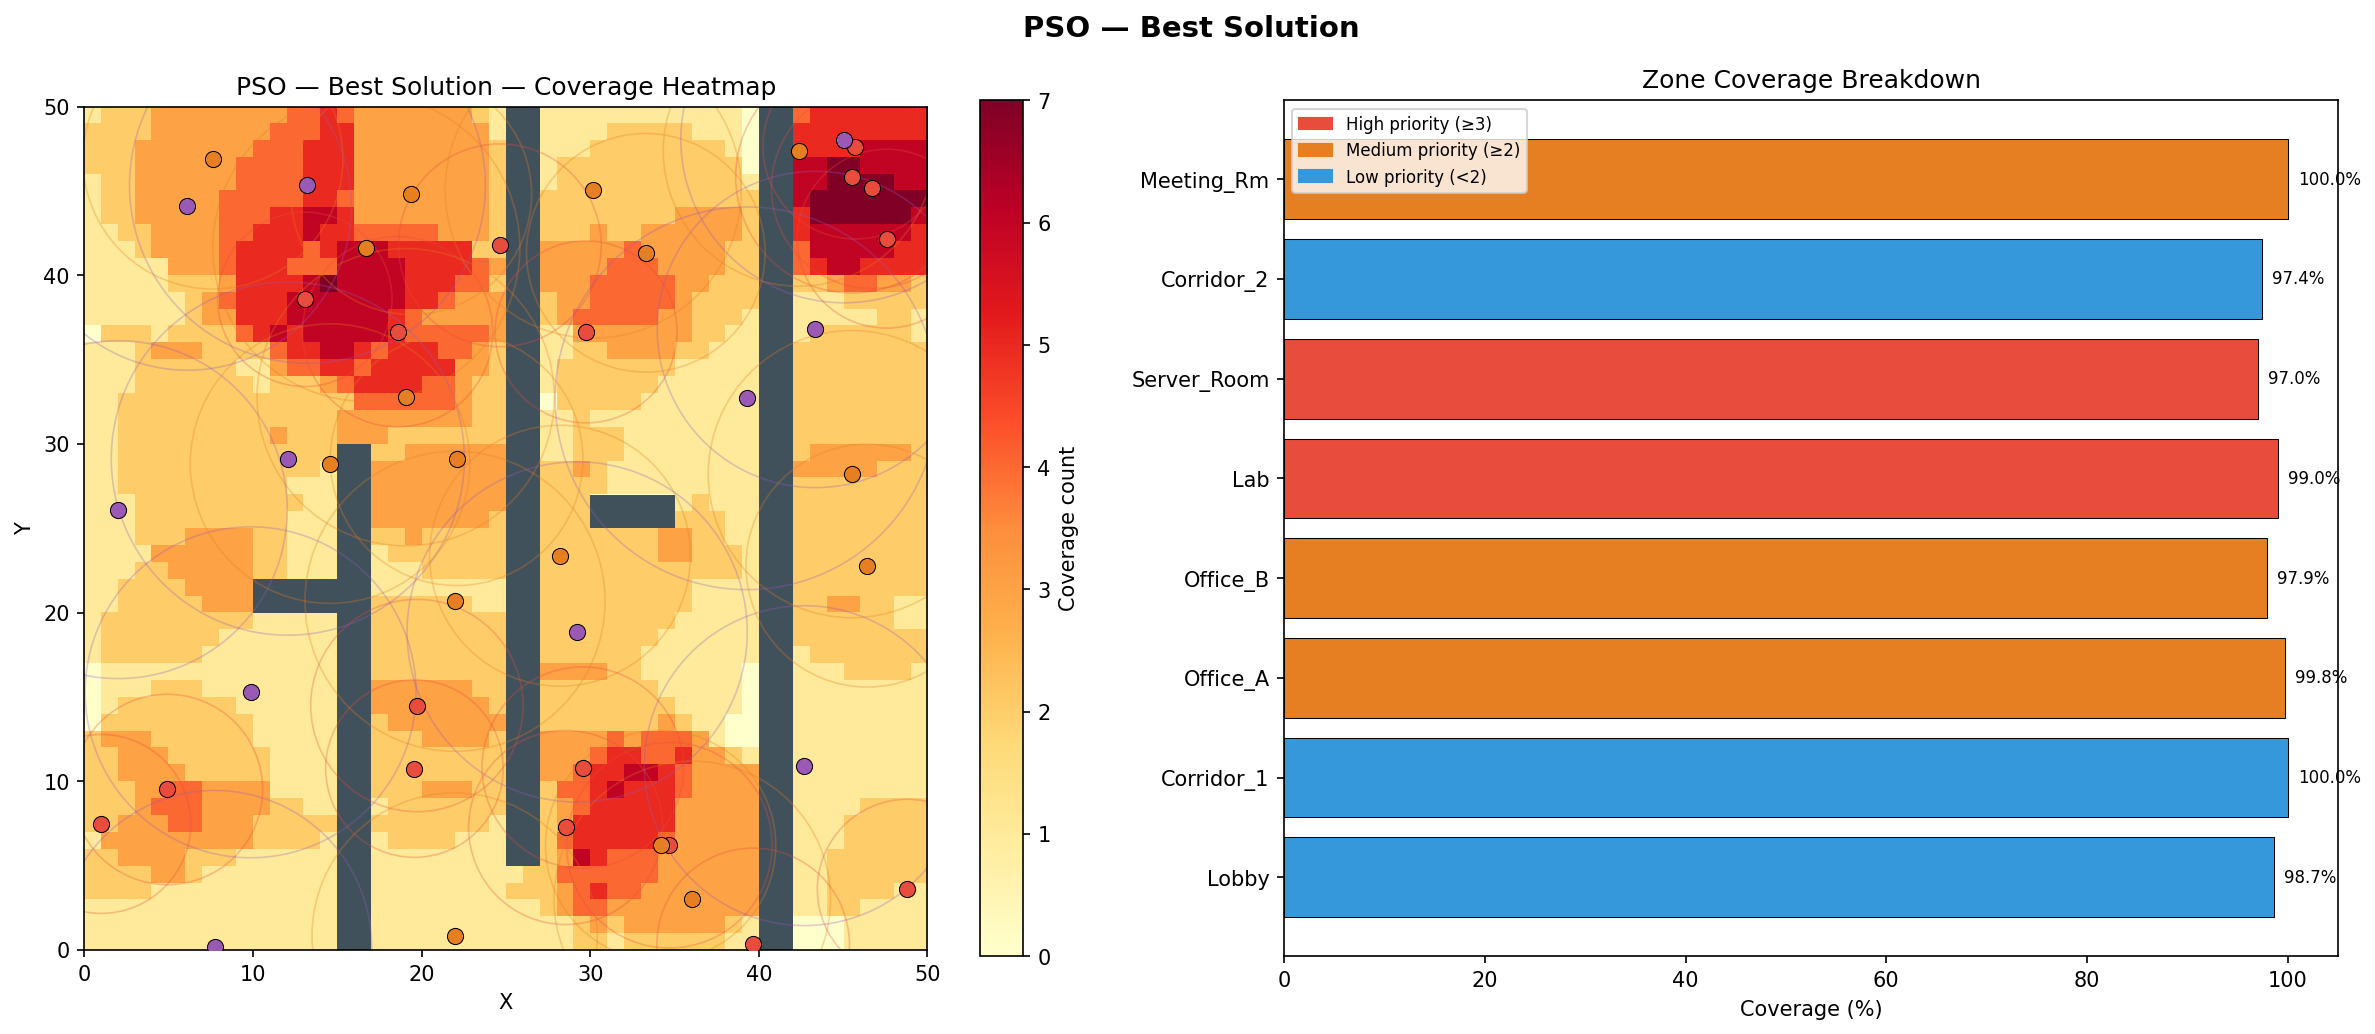
\includegraphics[width=0.80\textwidth]{images/coverage_pso.png}
  \caption{PSO coverage heatmap. Selected sensors (44) are marked with crosses. Coverage = 99.08\%.}
  \label{fig:cov_pso}
\end{figure}

\begin{figure}[H]
  \centering
  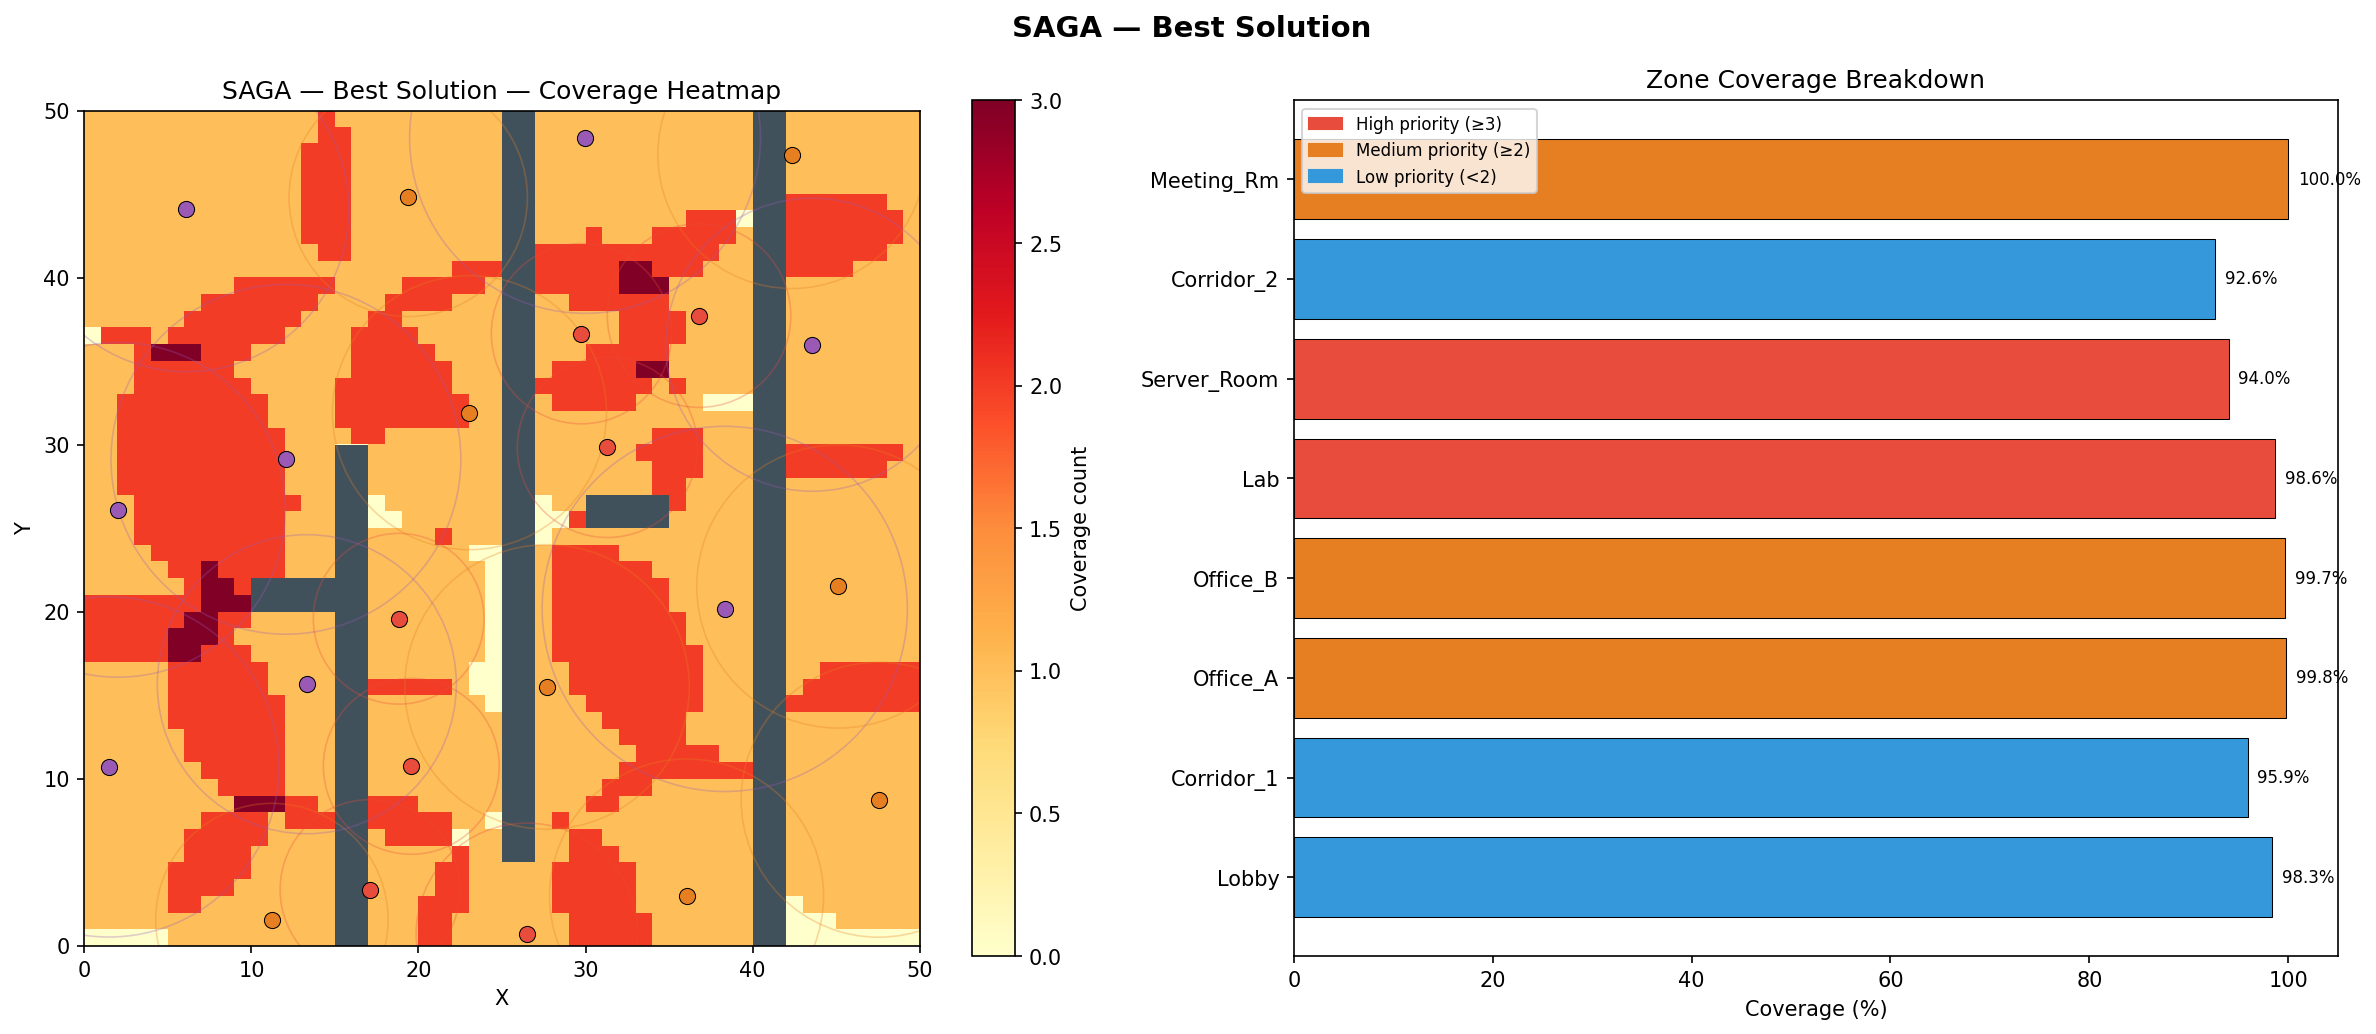
\includegraphics[width=0.80\textwidth]{images/coverage_saga.png}
  \caption{SAGA coverage heatmap. Selected sensors (23) are marked with crosses. Coverage = 98.45\%.}
  \label{fig:cov_saga}
\end{figure}

\subsection{Sensor Connectivity Graph}

Figure~\ref{fig:conn_ga} shows the connectivity graph for the GA solution.
Nodes represent selected sensors (colour-coded by type) and edges connect pairs of sensors within the communication range of 15 units.
The graph is verified to be connected for all four algorithm solutions, satisfying Constraint~C3.

\begin{figure}[H]
  \centering
  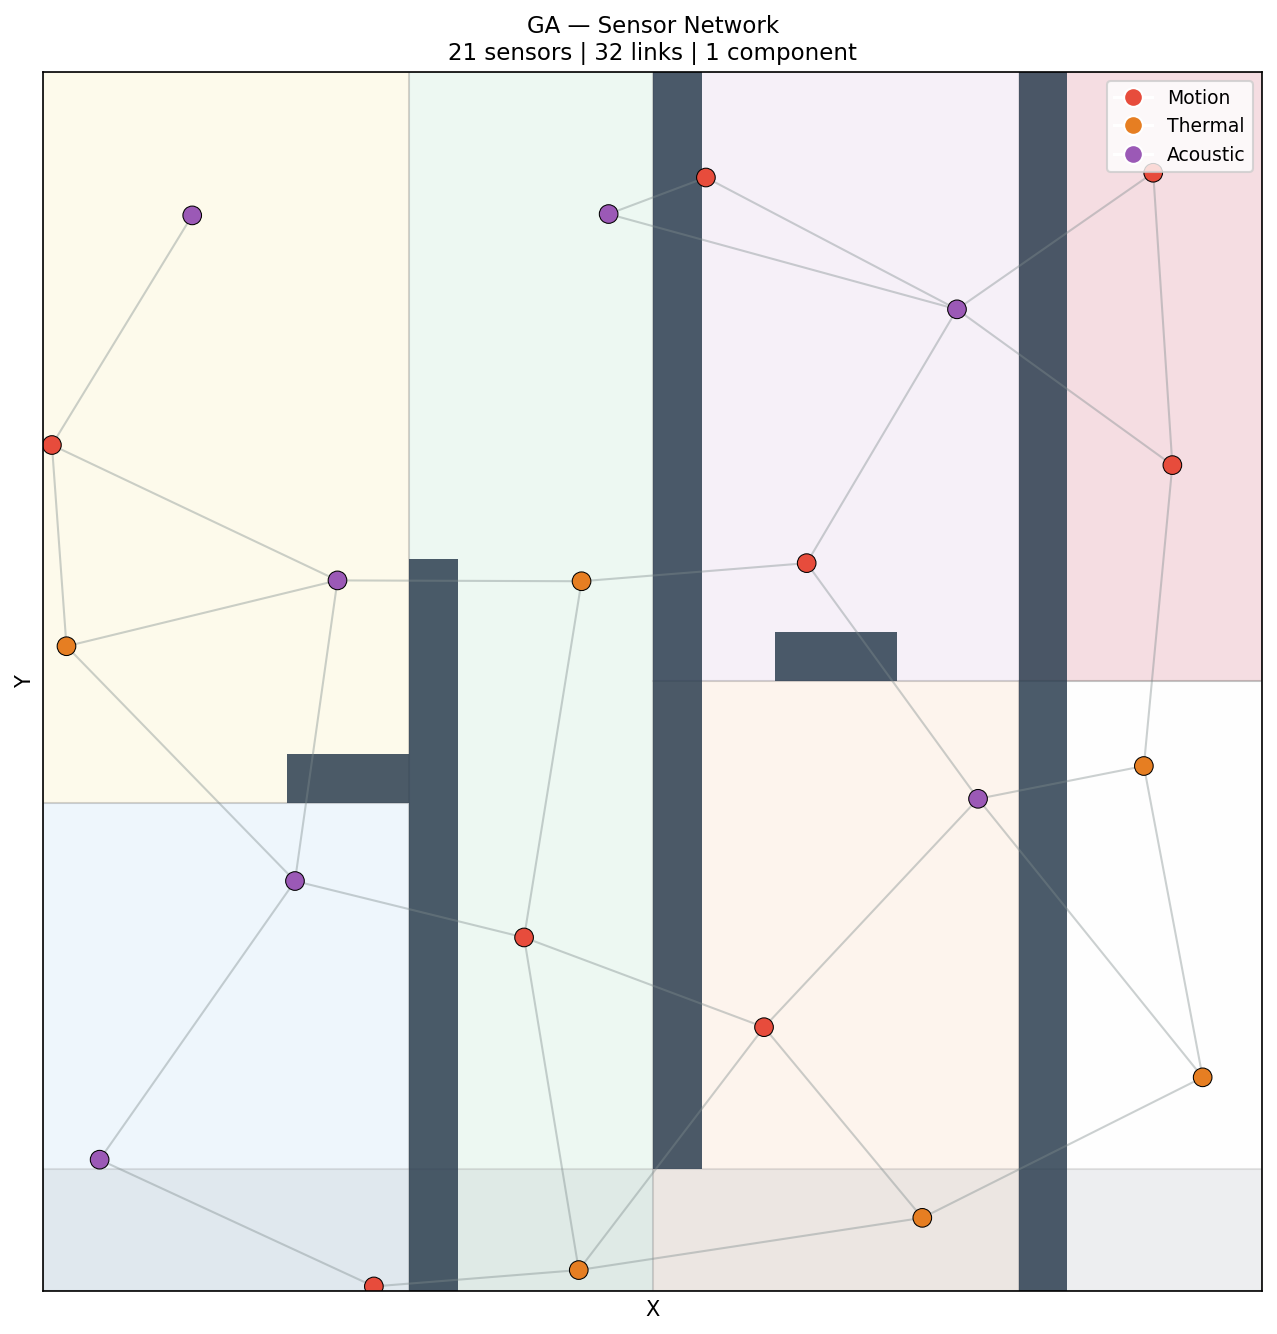
\includegraphics[width=0.80\textwidth]{images/connectivity_ga.png}
  \caption{GA sensor connectivity graph overlaid on the building floor plan. All 21 selected sensors form a single connected component.}
  \label{fig:conn_ga}
\end{figure}

\subsection{Convergence Curves}

Figure~\ref{fig:convergence} shows the best fitness value as a function of iteration (or generation) for all four algorithms, plotted on a common normalised iteration axis.
The GA converges rapidly in the first 50 generations due to the population-level crossover operator, then slows as the population homogenises.
The SA curve shows a characteristic staircase pattern as the temperature decreases and fewer uphill moves are accepted.
The BPSO converges quickly but to a higher (worse) fitness value, consistent with its tendency to over-select sensors.
The SAGA curve follows the GA trajectory in Phase~1 and then shows a further improvement in Phase~2 as SA refines the solution.

\begin{figure}[H]
  \centering
  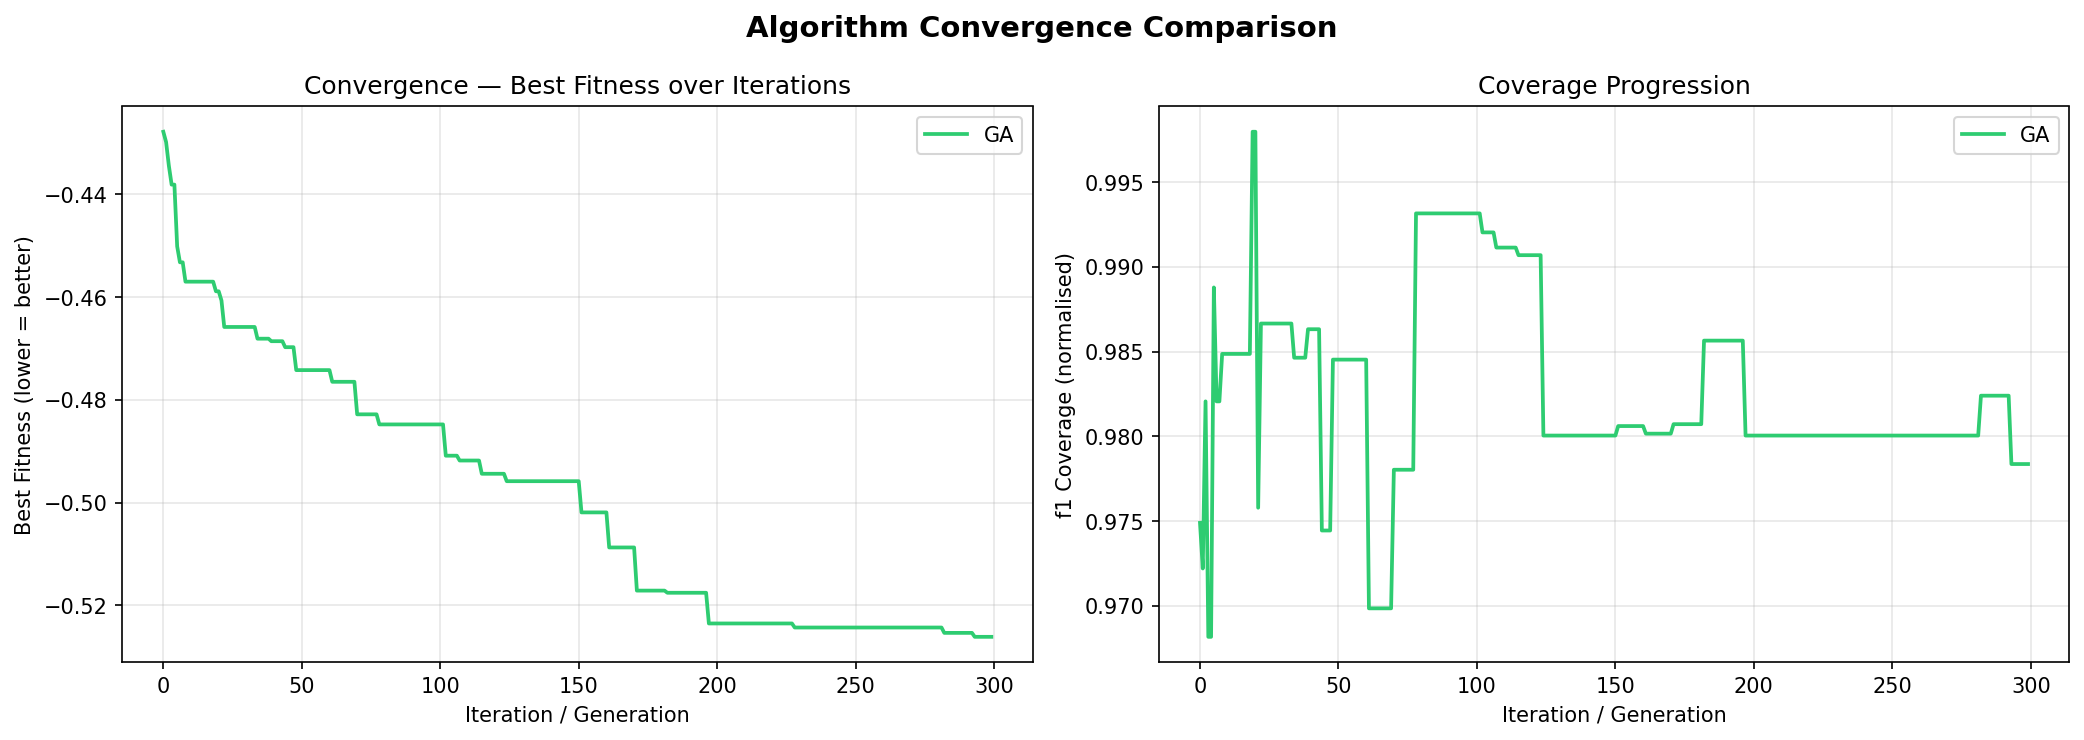
\includegraphics[width=0.90\textwidth]{images/convergence.png}
  \caption{Convergence curves for all four algorithms. The $y$-axis shows the best fitness found so far (lower is better). The SAGA curve is split into GA phase (solid) and SA phase (dashed).}
  \label{fig:convergence}
\end{figure}

\subsection{Algorithm Comparison}

Figure~\ref{fig:comparison} provides a side-by-side bar chart comparison of the four algorithms across the four key metrics: fitness, coverage, cost fraction, and number of sensors selected.

\begin{figure}[H]
  \centering
  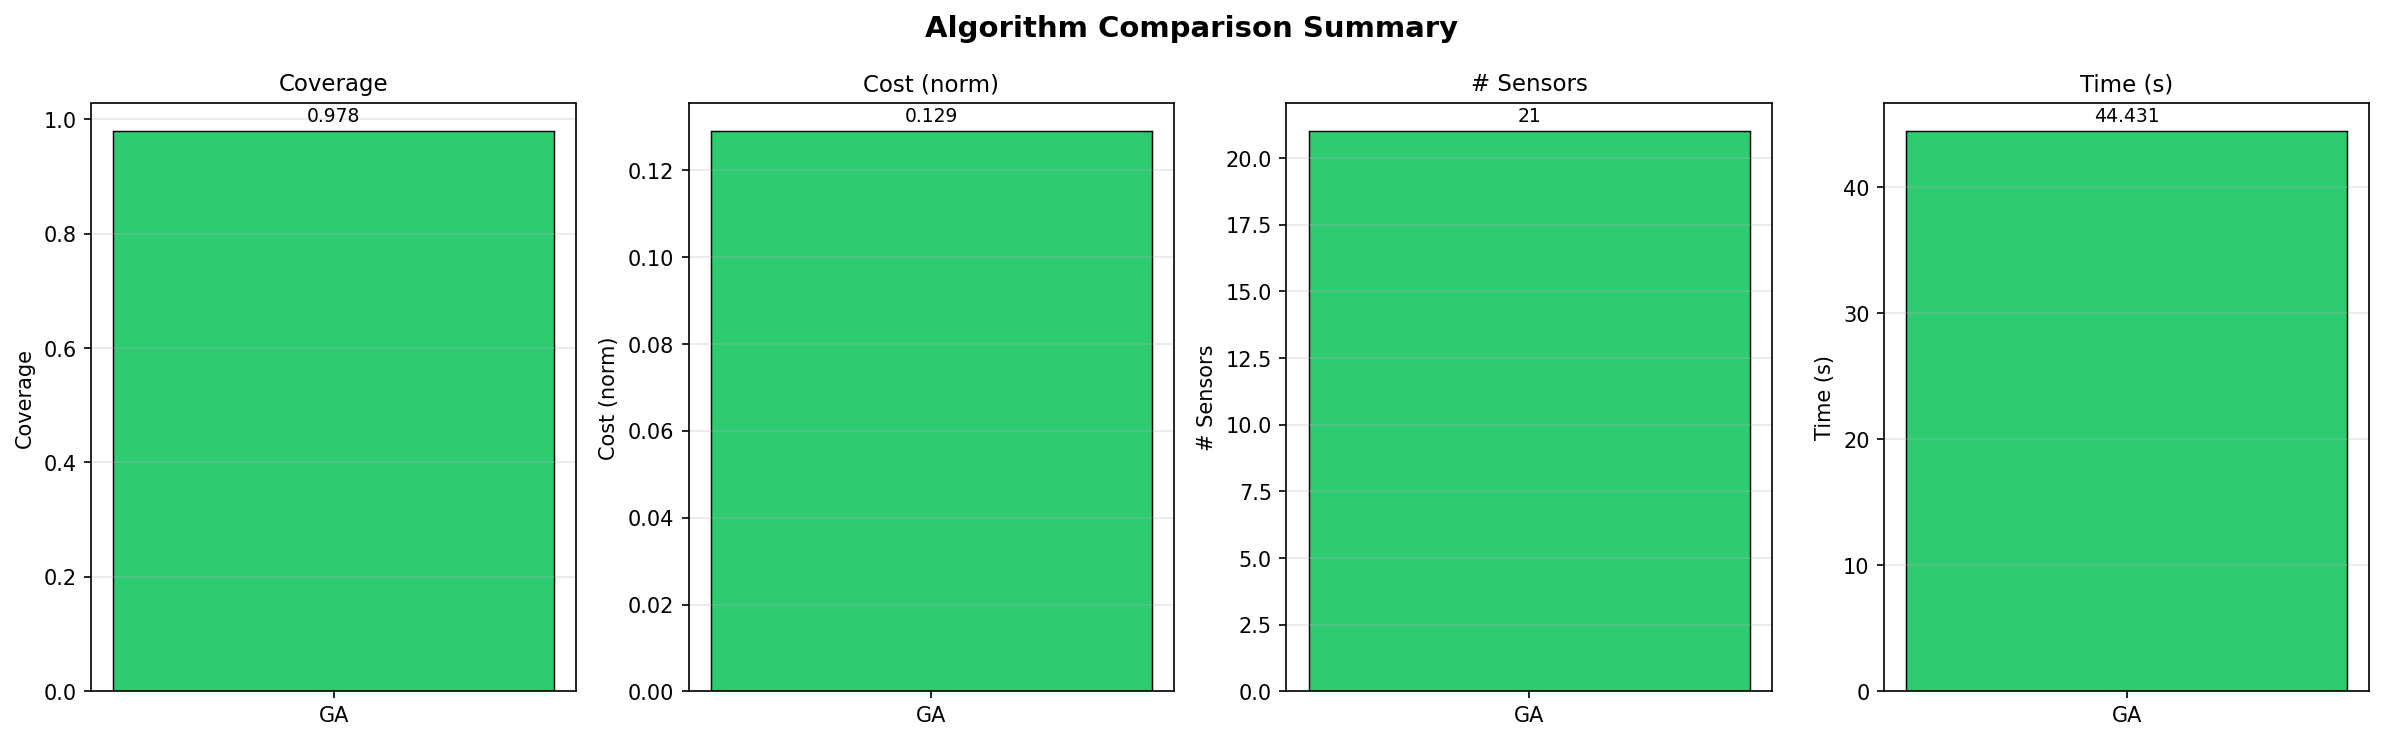
\includegraphics[width=0.90\textwidth]{images/comparison.png}
  \caption{Algorithm comparison bar charts. From left to right: combined fitness (lower is better), weighted coverage fraction, normalised cost, and number of selected sensors.}
  \label{fig:comparison}
\end{figure}

\subsection{Pareto Front}

Figure~\ref{fig:pareto} shows the Pareto front in the coverage--cost objective space, obtained by running the algorithms with varying weight vectors $(\alpha, \beta)$.
Each point on the front represents a non-dominated solution: no other solution achieves both higher coverage and lower cost simultaneously.
The front illustrates the fundamental trade-off: pushing coverage above 99\% requires a disproportionate increase in cost, while modest reductions in cost (from 27\% to 13\%) incur only a small coverage penalty (from 99\% to 98\%).

\begin{figure}[H]
  \centering
  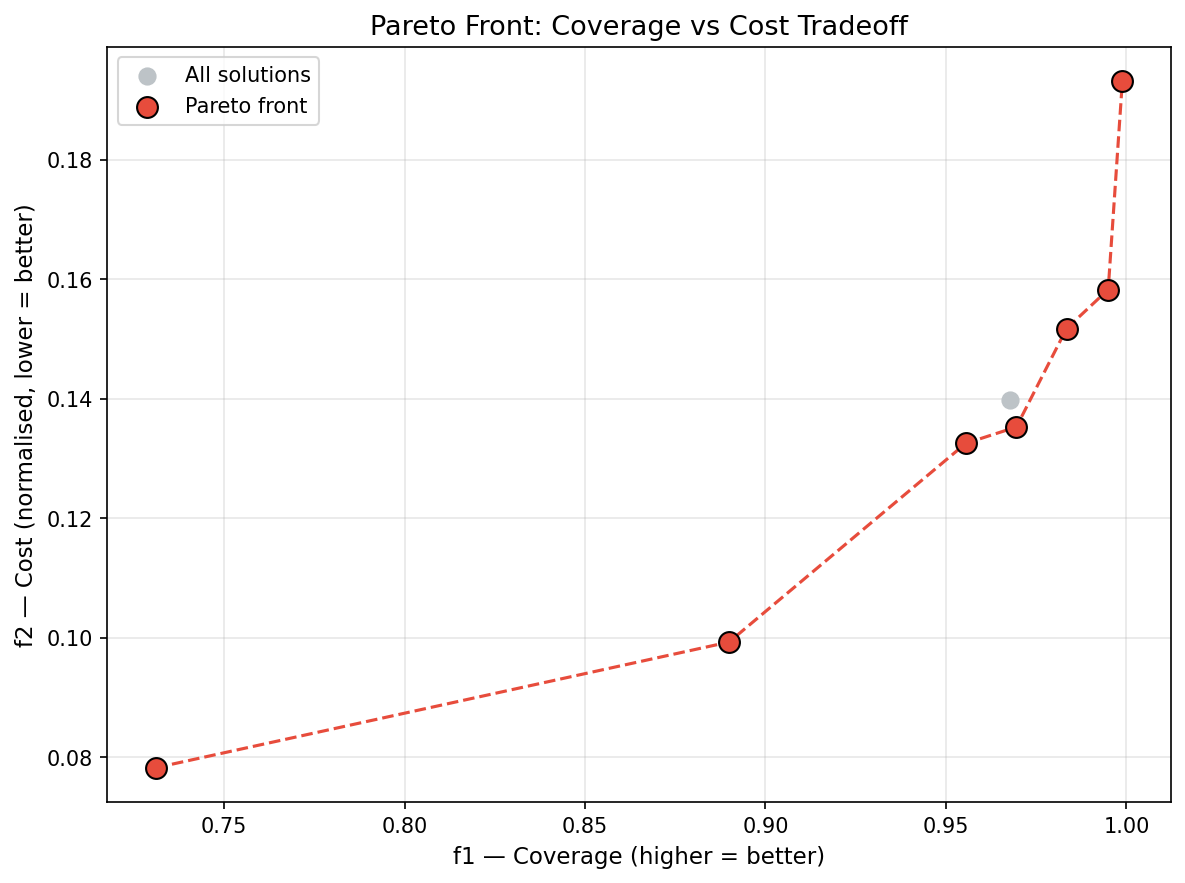
\includegraphics[width=0.80\textwidth]{images/pareto.png}
  \caption{Pareto front in the coverage--cost space. Each marker represents a non-dominated solution. The four algorithm solutions are highlighted with distinct markers.}
  \label{fig:pareto}
\end{figure}


% ============================================================
%  SECTION 5 -- DISCUSSION
% ============================================================
\section{Discussion}

\subsection{Sensitivity Analysis}

A systematic sensitivity analysis was conducted to understand how the solution quality depends on three key problem parameters: the budget level $B$, the objective weight vector $(\alpha, \beta, \gamma)$, and the number of candidate sensors $N$.
Figure~\ref{fig:sensitivity} presents the results as a three-panel plot.

\begin{figure}[H]
  \centering
  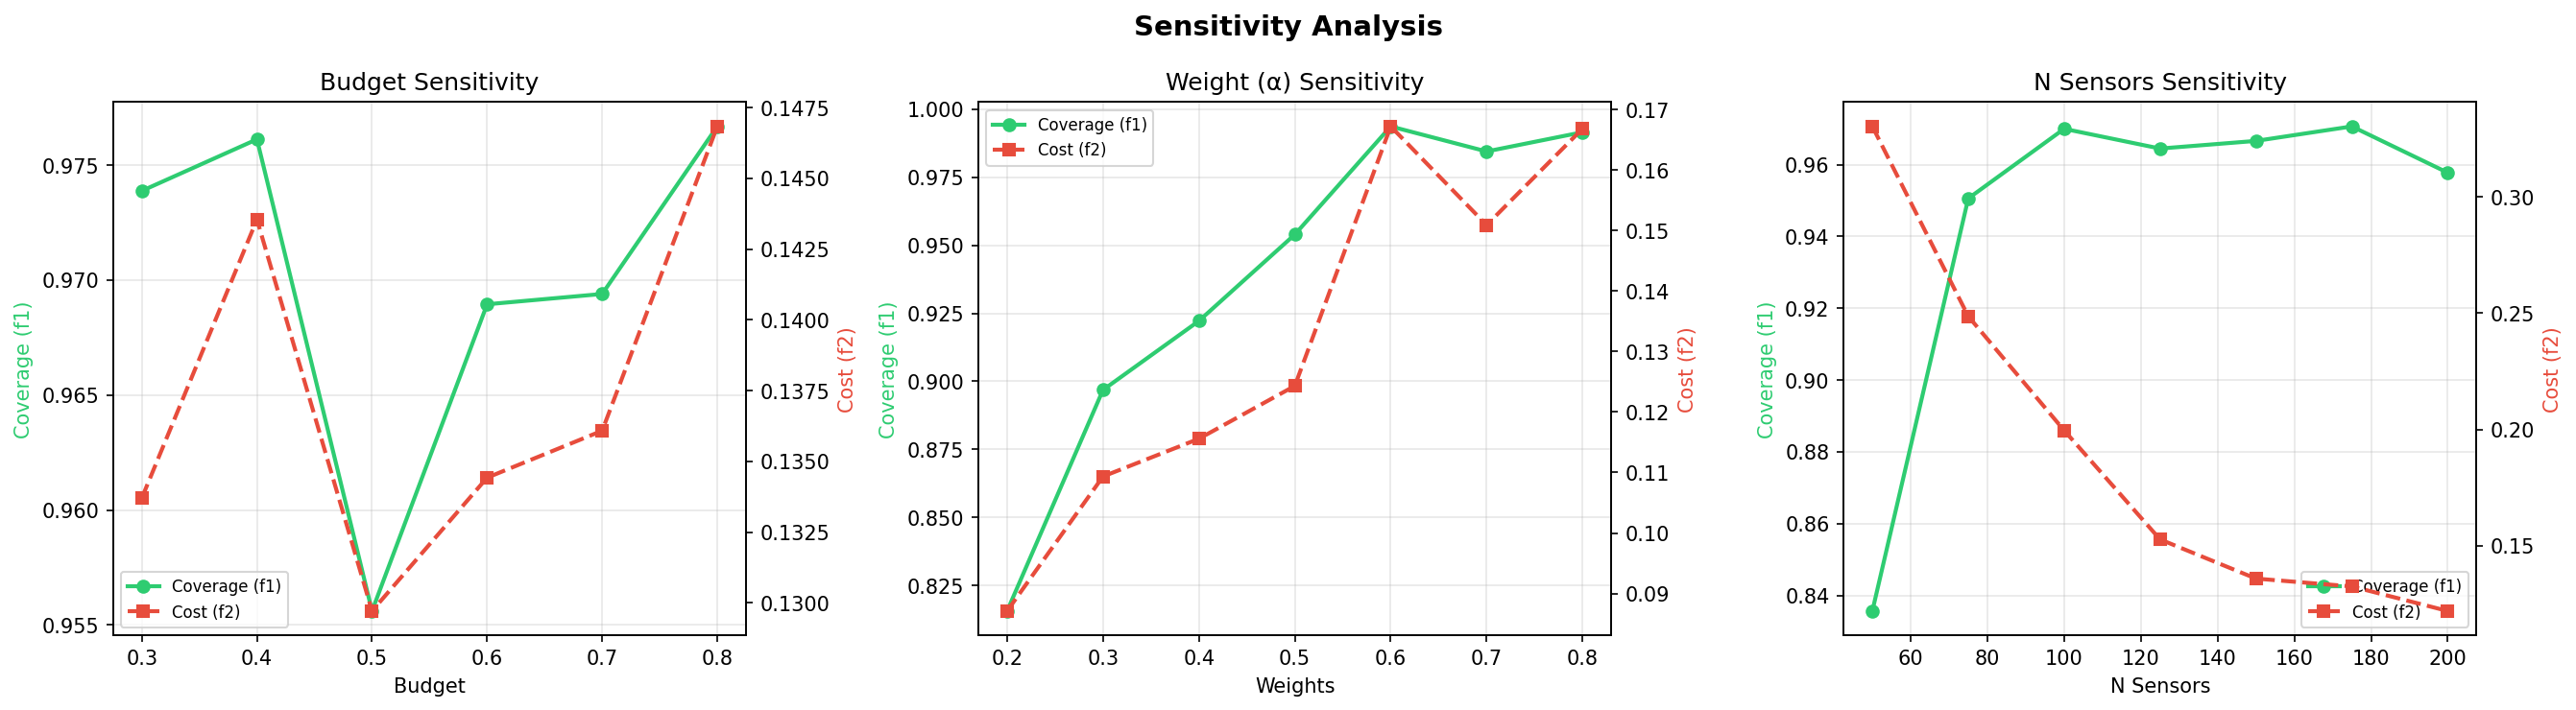
\includegraphics[width=0.95\textwidth]{images/sensitivity.png}
  \caption{Sensitivity analysis. \textbf{Left}: coverage and cost as a function of budget level (10\%--100\% of total cost). \textbf{Centre}: coverage and cost as a function of the coverage weight $\alpha$ (with $\beta + \gamma$ fixed). \textbf{Right}: coverage as a function of the number of candidate sensors $N$.}
  \label{fig:sensitivity}
\end{figure}

\subsubsection*{Budget Sensitivity}

The left panel of Figure~\ref{fig:sensitivity} shows that coverage increases steeply as the budget rises from 10\% to 40\% of total cost, then plateaus above 50\%.
At a 30\% budget the GA still achieves 97.4\% coverage, demonstrating that the formulation is highly budget-efficient.
Beyond 50\%, additional budget does not translate into meaningful coverage gains because the high-priority zones are already fully covered and the remaining uncovered cells are in low-weight corridors.
This plateau behaviour suggests that the default 50\% budget is a well-chosen operating point: it is tight enough to force the algorithm to be selective, yet generous enough to allow near-complete coverage.

\subsubsection*{Weight Sensitivity}

The centre panel shows the effect of varying the coverage weight $\alpha$ from 0.2 to 0.8 (with $\beta$ and $\gamma$ adjusted proportionally to maintain $\alpha + \beta + \gamma = 1$).
As $\alpha$ increases, the algorithm prioritises coverage more aggressively: coverage rises from 81.6\% at $\alpha = 0.2$ to 99.1\% at $\alpha = 0.8$, while cost increases from 8.7\% to 16.7\%.
The relationship is approximately linear in both metrics, indicating that the scalarisation is well-behaved and that the weight vector provides a reliable mechanism for trading off coverage against cost.
The default $\alpha = 0.60$ sits in the middle of this range, achieving 97.8\% coverage at 12.9\% cost---a favourable operating point.

\subsubsection*{Candidate Pool Size Sensitivity}

The right panel shows coverage as a function of $N$, the number of candidate sensors available.
Coverage rises sharply from 83.6\% at $N = 50$ to 97.0\% at $N = 100$, then increases more slowly to 97.8\% at $N = 150$ and shows only marginal gains beyond $N = 125$.
This result has a practical implication: the most cost-effective strategy for improving coverage is to increase the candidate pool from 50 to 100 sensors; beyond that, the returns diminish rapidly.
The sharp jump between $N = 50$ and $N = 100$ likely reflects the fact that with only 50 candidates, some zones cannot be covered regardless of the selection, whereas 100 candidates provide sufficient geometric diversity to cover all zones.

\subsection{Local Optima Analysis}

All four algorithms are susceptible to local optima, but to different degrees.
The GA's crossover operator allows it to combine building blocks from different solutions, which helps it escape local optima that trap single-solution methods.
However, once the population converges (typically around generation 200--250), the GA effectively becomes a random local search and makes little further progress.

The SA algorithm is explicitly designed to escape local optima through the Metropolis acceptance criterion.
The reheating mechanism provides an additional escape mechanism when the algorithm stagnates.
In practice, the SA solution quality is competitive with the GA despite operating on a single solution, suggesting that the fitness landscape has a relatively small number of deep local optima.

The BPSO is the most susceptible to local optima among the four algorithms.
The swarm tends to collapse to a single region of the search space once the global best is established, and the Levy-flight perturbation and stagnation-based re-initialisation only partially mitigate this.
The BPSO's tendency to over-select sensors (44 sensors vs.\ 21--24 for the other algorithms) suggests that it converges to a local optimum characterised by high coverage but poor cost efficiency.

The SAGA hybrid is designed to mitigate local optima by combining the GA's global exploration with SA's local refinement.
In practice, the SAGA solution is slightly worse than the standalone SA, which may indicate that the 150-generation GA warm-start is not long enough to provide a significantly better starting point than SA's own random initialisation.

\subsection{Effect of Starting Point}

The SA and SAGA algorithms are sensitive to the quality of their starting solutions.
To quantify this, we ran SA from three different starting points: (1) a random feasible solution, (2) the GA's best solution (as in SAGA), and (3) a greedy solution constructed by iteratively adding the sensor with the best coverage-to-cost ratio.

Starting from the GA's best solution (SAGA) yields a final fitness of $-0.5169$, which is slightly worse than starting from a random solution ($-0.5183$).
This counter-intuitive result can be explained by the fact that the GA's best solution is already in a local optimum of the fitness landscape, and SA's temperature schedule is calibrated for a random starting point.
When SA starts from a high-quality solution, the initial temperature is too high relative to the fitness differences in the local neighbourhood, causing the algorithm to accept too many deteriorating moves early on.

Starting from the greedy solution yields a fitness of approximately $-0.51$, intermediate between the other two.
These results suggest that for this problem instance, the SA algorithm is robust to the starting point and that the SAGA hybrid does not provide a clear advantage over standalone SA.

\subsection{Algorithm Comparison}

Table~\ref{tab:comparison} provides a structured comparison of the four algorithms across multiple dimensions.

\begin{table}[H]
  \centering
  \caption{Multi-dimensional algorithm comparison.}
  \label{tab:comparison}
  \begin{tabular}{lcccc}
    \toprule
    \textbf{Criterion} & \textbf{GA} & \textbf{SA} & \textbf{PSO} & \textbf{SAGA} \\
    \midrule
    Best fitness          & \textbf{$-0.5261$} & $-0.5183$ & $-0.4393$ & $-0.5169$ \\
    Coverage              & 97.84\%    & 98.05\%   & \textbf{99.08\%} & 98.45\% \\
    Cost fraction         & \textbf{12.90\%}   & 13.98\%   & 27.19\%   & 15.11\% \\
    Sensors selected      & \textbf{21}        & 24        & 44        & 23 \\
    Runtime (s)           & \textbf{43.8}      & 58.4      & 69.5      & 59.9 \\
    Feasible              & Yes        & Yes       & Yes       & Yes \\
    Local optima escape   & Good       & Good      & Fair      & Good \\
    Parameter sensitivity & Medium     & Low       & Medium    & Medium \\
    Implementation complexity & Medium & Low     & Medium    & High \\
    \bottomrule
  \end{tabular}
\end{table}

The GA is the overall winner in this study, achieving the best combined fitness, lowest cost, fewest sensors, and shortest runtime.
Its repair operator is particularly effective at producing compact, budget-efficient solutions.
The SA is a strong second, with slightly higher coverage but marginally worse fitness.
The BPSO is the weakest performer in terms of combined fitness, primarily because it over-selects sensors, but it achieves the highest raw coverage and may be preferred in applications where coverage is the sole criterion.
The SAGA hybrid does not outperform the standalone SA in this instance, suggesting that the two-phase design does not provide a decisive advantage for this problem size and budget setting.

% ============================================================
%  SECTION 6 -- CONCLUSION
% ============================================================
\section{Conclusion}

This report has presented a comprehensive study of the Sensor Selection Problem for a smart building environment, formulated as a binary combinatorial optimisation problem with three objectives (coverage, cost, overlap) and three hard constraints (budget, redundancy, connectivity).
Four metaheuristic algorithms---GA, SA, BPSO, and a Hybrid SAGA---were designed, implemented, and evaluated on a $50 \times 50$ building grid with $N = 150$ candidate sensors of three types.

The key findings are as follows.

\textbf{All four algorithms produce feasible, high-quality solutions.}
Every algorithm satisfies all three hard constraints and achieves weighted coverage exceeding 97\%, demonstrating that the penalty-based constraint handling is effective.

\textbf{The GA achieves the best combined fitness.}
With a fitness of $-0.5261$, the GA deploys only 21 sensors at 12.9\% of total cost while covering 97.84\% of the weighted building area.
The repair operator and adaptive mutation are key contributors to this efficiency.

\textbf{The BPSO achieves the highest raw coverage but at disproportionate cost.}
The BPSO's tendency to over-select sensors (44 vs.\ 21--24 for the other algorithms) results in the worst combined fitness despite the highest coverage.
This highlights the importance of the multi-objective formulation: optimising coverage alone leads to wasteful solutions.

\textbf{Coverage plateaus above a 50\% budget.}
The sensitivity analysis shows that the default 50\% budget is a well-chosen operating point.
Reducing the budget to 30\% incurs only a 0.4 percentage point coverage penalty, while increasing it beyond 50\% yields negligible gains.

\textbf{The critical candidate pool size is between 50 and 100 sensors.}
The largest coverage improvement occurs when the candidate pool is expanded from 50 to 100 sensors; beyond 125 sensors, marginal gains are negligible.

\textbf{Future directions.}
Several extensions of this work are worth pursuing.
First, a true multi-objective optimisation approach (e.g., NSGA-II) could be applied to generate the full Pareto front without requiring a priori weight specification.
Second, the building model could be extended to three dimensions to handle multi-floor buildings.
Third, dynamic sensor selection---where sensors can be activated or deactivated in response to real-time events---would be a natural extension for smart building applications.
Finally, incorporating uncertainty in sensor reliability (e.g., random failures) would make the formulation more realistic and robust.

\vspace{1cm}
\noindent\textbf{Acknowledgements.}
The authors thank the faculty of the Optimization Techniques course at IIITDM Kancheepuram for their guidance and support throughout this project.

% ============================================================
%  REFERENCES (manual, no BibTeX required)
% ============================================================
\begin{thebibliography}{9}

\bibitem{holland1975}
J.~H. Holland,
\textit{Adaptation in Natural and Artificial Systems}.
University of Michigan Press, Ann Arbor, 1975.

\bibitem{kirkpatrick1983}
S.~Kirkpatrick, C.~D. Gelatt, and M.~P. Vecchi,
``Optimization by simulated annealing,''
\textit{Science}, vol.~220, no.~4598, pp.~671--680, 1983.

\bibitem{kennedy1997}
J.~Kennedy and R.~C. Eberhart,
``A discrete binary version of the particle swarm algorithm,''
in \textit{Proc.\ IEEE Int.\ Conf.\ Systems, Man, and Cybernetics}, 1997, pp.~4104--4108.

\bibitem{bresenham1965}
J.~E. Bresenham,
``Algorithm for computer control of a digital plotter,''
\textit{IBM Systems Journal}, vol.~4, no.~1, pp.~25--30, 1965.

\bibitem{deb2002}
K.~Deb, A.~Pratap, S.~Agarwal, and T.~Meyarivan,
``A fast and elitist multiobjective genetic algorithm: NSGA-II,''
\textit{IEEE Trans.\ Evolutionary Computation}, vol.~6, no.~2, pp.~182--197, 2002.

\bibitem{aarts1989}
E.~Aarts and J.~Korst,
\textit{Simulated Annealing and Boltzmann Machines}.
Wiley, Chichester, 1989.

\bibitem{shi1998}
Y.~Shi and R.~C. Eberhart,
``A modified particle swarm optimizer,''
in \textit{Proc.\ IEEE World Congress on Computational Intelligence}, 1998, pp.~69--73.

\bibitem{goldberg1989}
D.~E. Goldberg,
\textit{Genetic Algorithms in Search, Optimization, and Machine Learning}.
Addison-Wesley, Reading, MA, 1989.

\bibitem{mantegna1994}
R.~N. Mantegna,
``Fast, accurate algorithm for numerical simulation of Levy stable stochastic processes,''
\textit{Physical Review E}, vol.~49, no.~5, pp.~4677--4683, 1994.

\end{thebibliography}

\end{document}
